\documentclass{beamercours}
\usepackage{tikzsymbols}
\usetikzlibrary{patterns, hobby}
\usetikzlibrary{shapes.callouts}
\usepackage{pgfplots}
\pgfplotsset{compat=1.6}

\begin{document}
\begin{frame}
\frametitle{Contextualisation}
\resizebox{\linewidth}{!}{

\begin{tikzpicture}[scale = .8, manstyle/.style={line width=4pt,line cap=round,line join=round}]
    \node[fill,circle,inner sep=2.5pt,outer sep=1pt] (head) at (-0.2mm,7.1mm) {}; 
    \node[above left,anchor=pointer,scale=0.4,cloud callout, cloud puffs=10, aspect=2, cloud puff arc=120,
    fill = blue!40!black,text=white,callout relative pointer={(-4mm,-4mm)}] at (2mm,8mm){Vanille};
    \draw[manstyle] (0,0.5) -- ++(0,-1.2cm);
\draw[manstyle] (-1.5pt,-1pt) -- ++(0,0.535cm) (1.2pt,1pt) --(0,5mm)--++(-80:5mm) coordinate (g);
\end{tikzpicture}
\hspace{-10pt}
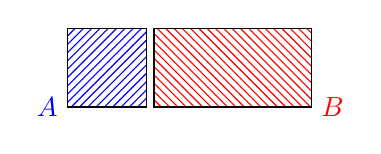
\begin{tikzpicture}
    \draw[pattern=north east lines, pattern color = blue] (0, 0) rectangle + (1, 1) ;
    \draw[blue] node[left] {$A$} (0, 0);
    \draw[pattern=north west lines, pattern color = red] (1.1, 0) rectangle + (2, 1) ;
    \draw[red] (3.1, 0) node[right] {$B$};
\end{tikzpicture}
\hspace{-10pt}

\begin{tikzpicture}[scale = .8, xscale = -1, manstyle/.style={line width=4pt,line cap=round,line join=round}]
    \node[fill,circle,inner sep=2.5pt,outer sep=1pt] (head) at (-0.2mm,7.1mm) {}; 
    \node[above left,anchor=pointer,scale=0.4,cloud callout, cloud puffs=10, aspect=2, cloud puff arc=120,
    fill = red!60!black,text=white,callout relative pointer={(4mm,-4mm)}] at (2mm,8mm){Chocolat};
    \draw[manstyle] (0,0.5) -- ++(0,-1.2cm);
\draw[manstyle] (-1.5pt,-1pt) -- ++(0,0.535cm) (1.2pt,1pt) --(0,5mm)--++(-80:5mm) coordinate (g);
\end{tikzpicture}}
\end{frame}


\begin{frame}
    \frametitle{}
    \resizebox{.8\textwidth}{!}{
        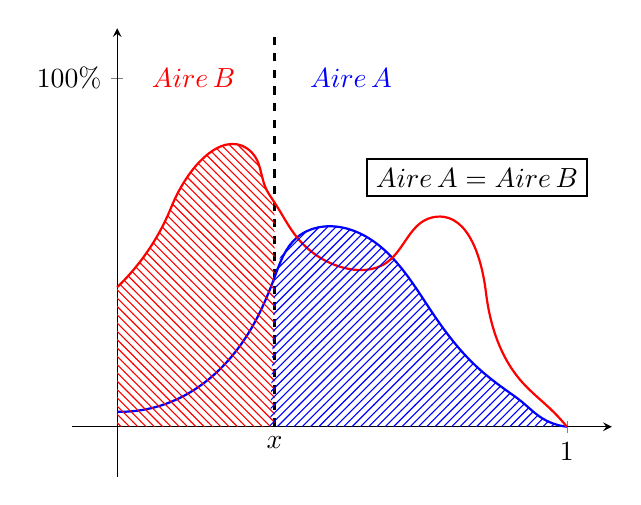
\begin{tikzpicture}
        \begin{axis}[
            xmin=-0.1,xmax=1.1,
            ymin=-0.1,ymax=.8,
            xtick={0, 1},
            xticklabels={$0$,$1$},
            ytick={0, .7},
            yticklabels={$0$,$100\%$},  
            axis lines=middle] 
        \draw[fill=none,thick,dashed] (axis cs:.35,0) node[below] {$x$} -- (axis cs:.35, 1.5);
        \draw[thick, blue] (axis cs:0, .03) to [curve through = { (axis cs:0.12, .05) .. (axis cs:0. 3, .2) .. (axis cs:0.35, .3) .. (axis cs:0.4, .38) .. (axis cs:0.5, .4) .. (axis cs:0.6, .35) .. (axis cs:0.7, .23) .. (axis cs:0.8, .12) .. (axis cs:0.87, .07) .. (axis cs:0.9, .05) .. (axis cs:0.94, 0.02)}] (axis cs:1., 0.);
        \draw[thick, red] (axis cs:0, .28) to [curve through = { (axis cs:0.12, .44) .. (axis cs:0.3, .55) .. (axis cs:0.33,.48) .. (axis cs:0.35, .45) .. (axis cs:0.4, .38) .. (axis cs:0.5, .32) .. (axis cs:0.6, .33) .. (axis cs:0.7, .42) .. (axis cs:0.82, .27) .. (axis cs:0.9, .09) .. (axis cs:0.97, .03) }] (axis cs:1, 0);
        \draw[draw = none, pattern = north west lines, pattern color = red] (axis cs:0, 0) to (axis cs:0, .28) to [curve through = { (axis cs:0.12, .44) .. (axis cs:0.3, .55) .. (axis cs:0.33,.48)}] (axis cs:.35, .44) to (axis cs:.35, 0);
        \draw[draw = none, pattern = north east lines, pattern color = blue] (axis cs:0.34, 0) to (axis cs:0.35, .3) to [curve through = {(axis cs:0.4, .38) .. (axis cs:0.5, .4) .. (axis cs:0.6, .35) .. (axis cs:0.7, .23) .. (axis cs:0.8, .12) .. (axis cs:0.87, .07) .. (axis cs:0.9, .05) .. (axis cs:0.94, 0.02)}] (axis cs:1, 0);
        \draw[thick] (axis cs:0.17, .7) node[thick, red] {$\mathop{Aire } B$};
        \draw[thick] (axis cs:0.52, .7) node[thick, blue] {$\mathop{Aire } A$};
        \draw[thick] (axis cs:.8,.5) node[rectangle, draw = black] {$\mathop{Aire } A = \mathop{Aire } B$};
        \end{axis}
    \end{tikzpicture}}
\end{frame}


\end{document}
